% Source: 2006 Fujian science candidate PDF, source ID
% src-ab0f2729ee4a24495e653b44c14438b4130f8b38b11362bf84251f3595a09d27,
% SHA-256 50d17546b94af82fb2cee653942752914cd387fe72792d74ffa5f75e7a301d83,
% page 1, printed page 288, Q16. Schematic reconstruction; not a measurement drawing.
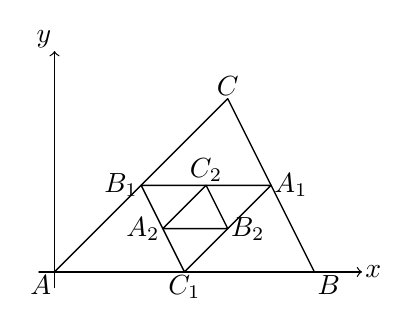
\begin{tikzpicture}[x=1.1cm,y=1.1cm,line cap=round,line join=round]
  \coordinate (A)  at (0,0);
  \coordinate (B)  at (3,0);
  \coordinate (C)  at (2,2);
  \coordinate (A1) at (2.5,1);
  \coordinate (B1) at (1,1);
  \coordinate (C1) at (1.5,0);
  \coordinate (A2) at (1.25,0.5);
  \coordinate (B2) at (2,0.5);
  \coordinate (C2) at (1.75,1);

  % Coordinate axes shown in the source diagram.
  \draw[->,line width=0.45pt] (0,-0.18) -- (0,2.55);
  \draw[->,line width=0.45pt] (-0.18,0) -- (3.55,0);

  % Original triangle and the first two midpoint triangles.
  \draw[line width=0.5pt] (A)--(B)--(C)--cycle;
  \draw[line width=0.5pt] (A1)--(B1)--(C1)--cycle;
  \draw[line width=0.5pt] (A2)--(B2)--(C2)--cycle;

  \node[below left,inner sep=1pt]  at (A)  {$A$};
  \node[below right,inner sep=1pt] at (B)  {$B$};
  \node[above,inner sep=1pt]       at (C)  {$C$};
  \node[right,inner sep=1pt]       at (A1) {$A_1$};
  \node[left,inner sep=1pt]        at (B1) {$B_1$};
  \node[below,inner sep=1pt]       at (C1) {$C_1$};
  \node[left,inner sep=1pt]        at (A2) {$A_2$};
  \node[right,inner sep=1pt]       at (B2) {$B_2$};
  \node[above,inner sep=1pt]       at (C2) {$C_2$};
  \node[above left,inner sep=1pt]  at (0,2.55) {$y$};
  \node[right,inner sep=1pt]       at (3.55,0) {$x$};
\end{tikzpicture}
